
\documentclass[11pt,a4paper]{article}
\usepackage[margin=2.4cm]{geometry}
\usepackage{amsmath,amssymb}
\usepackage{siunitx}
\usepackage{booktabs}
\usepackage{graphicx}
\usepackage{microtype}
\usepackage[font=small,labelfont=bf]{caption}
\usepackage{xcolor}
\usepackage[hidelinks,
  pdftitle={A three-objective optimisation framework for circular product ecodesign, built end to end on open data},
  pdfauthor={Adeleke Olorunnisola},
  pdfsubject={Multi-objective optimisation for circular product ecodesign},
  pdfkeywords={circular economy, ecodesign, NSGA-III, life cycle assessment, multi-objective optimisation}
]{hyperref}
\usepackage{enumitem}
\usepackage{titlesec}
\usepackage{placeins}
\renewcommand{\topfraction}{0.92}
\renewcommand{\bottomfraction}{0.75}
\renewcommand{\textfraction}{0.06}
\renewcommand{\floatpagefraction}{0.80}
\setcounter{topnumber}{3}
\setcounter{totalnumber}{5}
\titleformat{\section}{\large\bfseries}{\thesection}{0.7em}{}
\titleformat{\subsection}{\normalsize\bfseries}{\thesubsection}{0.6em}{}
\setlist{itemsep=1pt,topsep=3pt}
\renewcommand{\arraystretch}{1.12}

\title{\Large\textbf{A three-objective optimisation framework for circular product\\
ecodesign, built end to end on open data}}
\author{Adeleke Olorunnisola}
\date{}

\begin{document}
\maketitle

\begin{abstract}
\noindent
Circular ecodesign stalls at the concept stage because designers cannot show
that circularity will eventually yield profit. This report builds a framework that decides the
question quantitatively for one product: the GARO LS4 ground-mounted AC
electric-vehicle charging station, whose bill of materials, mass and service
life are taken from a published manufacturer LCA rather than assumed.
Fourteen design variables (recycled
content, joining method, design life, number of remanufacture cycles,
end-of-life route per material family and standby power class) are
optimised simultaneously against three objectives: cradle-to-grave carbon per
service-year (\emph{Planet}), annualised life-cycle cost (\emph{Prosperity}),
and a composite repairability, modularity, circular-labour and supply-risk
index (\emph{People}). The life-cycle inventory is read at run time from the
Idemat 2026, a process-level inventory carrying global warming, cumulative
energy demand and the European Commission's Environmental Footprint 3.1
method; commodity prices come from the USGS Mineral Commodity Summaries 2025
(US public domain). No licensed database is used and no factor is invented.
Every methodological choice that could decide the answer is tested rather than
assumed: impact category, end-of-life allocation convention (including the EU
Product Environmental Footprint's own Circular Footprint Formula), grid
geography, social weighting, price source, the electronics proxy, the three
unmeasured recyclate constants, and the widths of the scenario distributions.
One of those tests overturns a comfortable assumption: purely methodological
choices routinely move the Planet objective more than the entire Pareto
archive of design decisions does, which is reported as a finding in its own
right, not smoothed over. A
self-contained NSGA-III recovers a 359-design Pareto
archive, of which 359
designs beat a linear take-make-waste baseline on carbon \emph{and} cost at
the same time: the central claim, and the one industry disputes. A
Monte-Carlo ensemble of 500 futures, spanning grid
decarbonisation, carbon pricing, commodity volatility observed in the USGS
series, remanufacturing performance and an ESPR-style minimum recycled-content
mandate, then separates designs that are merely optimal today from designs
that stay good answers under uncertainty. 55 of
359 designs survive that test. Reading the same front
through four decision-maker preference profiles produces
3 distinct recommendations, which is the practical
content of the exercise: the front is one artefact, the decision is not.
\end{abstract}

\section{Why this problem}

Circular economy has more definitions than consensus: a review of 114
published definitions found that most reduce it to reduce/reuse/recycle
activity and rarely connect it to social equity at all [24]. That gap is one
reason the People objective in this framework is a full, independently
optimised objective rather than a constraint bolted onto an environmental
model, following the Life Cycle Sustainability Assessment framing of
LCA + LCC + S-LCA as three co-equal pillars, not one pillar with two
footnotes [22].

The European Ecodesign for Sustainable Products Regulation moves circularity
from voluntary to mandatory [11], and the Digital Product Passport it
introduces will make the underlying data auditable at end of life in a way
existing WEEE take-back schemes were not designed for [27]. The barrier is no
longer intent. It is
that deep circularity (designing for disassembly, remanufacturing,
high-purity recycling) demands capital up front against benefits that are
distributed across a decade, split between actors, and exposed to commodity
and regulatory volatility. A product manager asked to approve a snap-fit
tooling premium today, for a scrap revenue in 2038, has no rigorous way to
answer.

Existing eco-efficiency tools answer a narrower question. They optimise one
variable, hold the rest fixed, evaluate against today's factors, and collapse
the social dimension into a footnote. That produces recommendations which are
locally correct and strategically useless.

This work takes the opposite stance on three points.

\begin{enumerate}
\item \textbf{Three objectives, not one.} Planet, Prosperity and People are
kept separate to the end. Aggregating them early hides exactly the trade-off
the decision-maker is paid to make.
\item \textbf{Futures, not a snapshot.} A design is scored by how often it is
a good answer across an ensemble of futures, not by its rank against today's
factors.
\item \textbf{Provenance, not precision theatre.} Every quantity is tagged
\textsc{data}, \textsc{proxy} or \textsc{assumption}. The proxies and
assumptions are perturbed hardest in the scenario ensemble, so the reader can
see which conclusions rest on measurement and which rest on judgement.
\end{enumerate}

\section{Data}

Three datasets are used. Two are freely redistributable without restriction;
the third is free to use with attribution and is fetched rather than
redistributed.

\paragraph{Idemat 2026} (Vogtlander, Sustainability Impact Metrics / Delft
University of Technology) is the life-cycle inventory. It is process-level,
which matters for two reasons beyond the obvious one.

First, it carries a full impact-assessment layer, so the same calculation
yields global warming, cumulative energy demand, the European Commission's
Environmental Footprint 3.1 single score and the EF 3.1 minerals-and-metals
score simultaneously. EF 3.1 is the method the ESPR delegated acts are written
against, which makes it the right yardstick for a study framed around that
regulation.

Second, and more importantly for a circularity study, it resolves \emph{process
pairs}: primary and secondary production of the same material, and end-of-life
processes carrying explicit substitution credits. Recycled content is therefore
a blend between two real production routes rather than a ratio between two
reporting factors, and the end-of-life credit convention becomes a choice this
study can test rather than one the dataset imposes.

Which Idemat process represents which material family is a modelling decision,
not a parsing detail, so it lives in
\texttt{data/idemat\_process\_map.json} with a justification per entry and a
resolver that fails loudly if a code moves between releases. Process choice is
decided per family on the evidence available rather than by a blanket rule:
grid electricity uses the European (Swedish) region, matching the factory's
location, which is the one geographic fact this study is actually sure of.
Material \emph{production} routes are not assumed to follow the factory
location by default: aluminium in particular defaults to the
\emph{global-average} primary route, because GARO's own published transport
data shows an internationally distributed supplier base and no source names a
specific smelter. Section~\ref{sec:validation} and the geography
reconciliation in Section~9 set out the evidence and test the alternative.

\paragraph{UK Government GHG Conversion Factors for Company Reporting 2025}
(DESNZ/DEFRA, Open Government Licence v3.0) is retained as a second,
independent backend rather than discarded. It is a corporate GHG-reporting
dataset, not a life-cycle inventory: single-issue, built on consumer waste
categories, and carrying no avoided-burden credit at end of life. Keeping it
selectable means the two can be compared, which is how the earlier version
of this study, built on DEFRA alone, can be shown to have been carbon
footprinting rather than LCA.

\paragraph{USGS Mineral Commodity Summaries 2025} salient-statistics data
releases (US Geological Survey; a work of the US Government, public domain).
These supply annual average commodity prices for the life-cycle costing, and,
more usefully, a five-year price history per commodity. That history
is put to two uses: it calibrates the price shocks in the scenario ensemble,
and its coefficient of variation is used as an observable proxy for supply
risk in the People objective, so the social weighting of recycled content is
derived from data rather than asserted.

\begin{table}[t]
\centering\small
\caption{Life-cycle inventory factors, as parsed from the DEFRA 2025 workbook at
run time. \textsc{data} means the material family maps directly onto a
published row; \textsc{proxy} means the closest published material is used as
a stand-in and the scenario ensemble perturbs it hardest.}
\label{tab:factors}
\begin{tabular}{llp{6.0cm}rrr}
\toprule
family & tag & DEFRA material & primary & closed-loop & cut \\
 & & & \multicolumn{2}{c}{kg CO$_2$e/kg} & \% \\
\midrule
plastic & \textsc{data} & Plastics: average plastic rigid & 3.354 & 1.916 & 42.9 \\
steel & \textsc{proxy} & Metal: steel cans & 2.864 & 1.824 & 36.3 \\
aluminium & \textsc{proxy} & Metal: aluminium cans and foil (excl. forming) & 9.116 & 0.995 & 89.1 \\
copper & \textsc{proxy} & Metal: scrap metal & 3.473 & 1.706 & 50.9 \\
electronics & \textsc{proxy} & Electrical items - IT & 24.866 & -- & -- \\
\bottomrule
\end{tabular}
\end{table}

\begin{table}[t]
\centering\small
\caption{Commodity prices parsed from the USGS MCS 2025 salient-statistics
releases. Unit conversion is driven by the column-name suffix
(\texttt{ctslb}, \texttt{dt}, \texttt{dtoz}).}
\begin{tabular}{llrrl}
\toprule
commodity & as published & year & USD/kg & source column \\
\midrule
Copper & 430.0 cents/lb & 2024 & 9.480 & \texttt{Price\_US\_ctslb} \\
Iron and Steel Scrap & 325.0 USD/t & 2024 & 0.325 & \texttt{Price\_Num\_1\_heavy\_dt} \\
Nickel & 17000.0 USD/t & 2024 & 17.000 & \texttt{Price\_dt} \\
Silver & 27.7 USD/troy oz & 2024 & 890.576 & \texttt{Price\_Bullion\_dtoz} \\
Tin & 1400.0 cents/lb & 2024 & 30.865 & \texttt{Price\_NY\_ctslb} \\
Zinc & 144.0 cents/lb & 2024 & 3.175 & \texttt{Price\_ctslb} \\
\bottomrule
\end{tabular}
\end{table}

\paragraph{What the data does not cover.} Three gaps are load-bearing and are
declared rather than papered over. First, no open dataset gives an engineering
polymer price index, so the PC/ABS resin price is an assumption. Second, the
USGS aluminium release was not retrievable during this run, so its price falls back to a declared assumption.
Third, DEFRA does not resolve copper or populated electronics as materials;
both use proxies, which is why they carry the widest uncertainty
($\sigma=0.35$ lognormal) in the ensemble. A model that hid these would report
the same numbers with false confidence.

\begin{figure}[t]
\centering
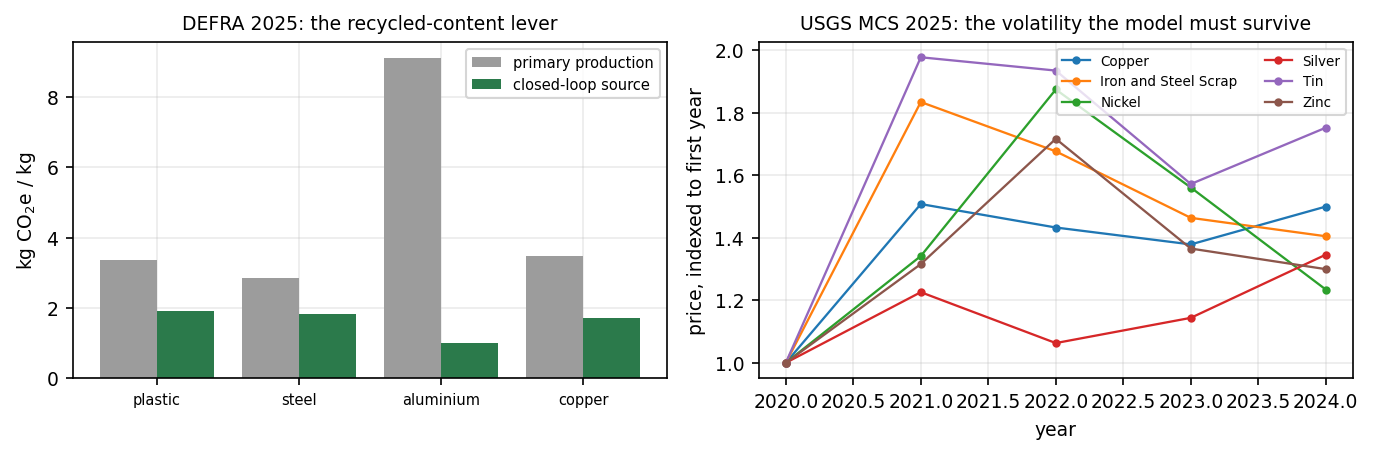
\includegraphics[width=\textwidth]{figures/fig_datasets.png}
\caption{Left: the recycled-content lever, straight from DEFRA 2025: the gap
between the two bars is the entire environmental case for secondary material.
Right: USGS price histories, indexed to 2020. The dispersion on the right is
why a single-point-in-time optimisation is not a decision aid.}
\end{figure}

\FloatBarrier
\section{Product and design space}

The case product is the GARO LS4, a ground-mounted AC electric-vehicle
charging station of total mass \SI{24.50}{\kilo\gram}.
It sits inside ESPR scope, has a substantial use phase, and has the modular
architecture that makes disassembly decisions meaningful.

It was chosen for one reason above the others: \emph{its bill of materials is
published}. Persson and Erselius [1] report, for this exact unit,
the material distribution by mass, the \SI{24.5}{\kilo\gram} product mass,
the \SI{29.7}{\kilo\gram} mass including packaging, a 15-year technical
life and 20\,000 charging sessions over that life. The mass basis of every
number in this report is therefore citable rather than invented, which
matters, because a life-cycle model is only ever as defensible as the
inventory it multiplies.

Two things remain this project's own. Packaging (corrugated cardboard,
laminated paper and paper, 16\,\% of the published bill of materials)
is excluded and the remainder renormalised onto the official product mass.
And the report publishes mass by \emph{material}, not by component, so the
split of each material total across components is an assumption, declared
in \texttt{data/garo\_ls4\_bom.json} and constrained so that the family
totals reproduce the published percentages exactly. The regression suite
fails if that constraint is ever broken.

\begin{table}[h]
\centering\small
\caption{Bill of materials. \emph{Priority repair} marks the components a
repairer must reach; \emph{interface} indexes the joining decision that governs
access.}
\begin{tabular}{lrllc}
\toprule
component & mass (kg) & family & priority repair & interface \\
\midrule
aluminium door / front panel & 4.19 & aluminium & no & 0 \\
aluminium pedestal extrusion & 8.51 & aluminium & no & 0 \\
aluminium internal chassis and heat spreader & 1.91 & aluminium & no & 1 \\
main contactor & 1.10 & electronics & yes & 1 \\
control and metering PCBA & 1.30 & electronics & yes & 1 \\
RCD / RCM module & 0.60 & electronics & yes & 1 \\
power and EMC board & 1.30 & electronics & yes & 1 \\
cable copper conductor & 1.15 & copper & no & 2 \\
cable sheath & 1.15 & plastic & no & 2 \\
steel mounting base plate & 1.20 & steel & no & 1 \\
fasteners and small steel parts & 0.52 & steel & no & -- \\
internal mouldings and covers & 0.84 & plastic & no & 1 \\
connector housing & 0.55 & plastic & no & 2 \\
gaskets and seals & 0.19 & plastic & no & 0 \\
\midrule
\textbf{total} & \textbf{24.50} & & & \\
\bottomrule
\end{tabular}
\end{table}

The design vector has 3 continuous and 11 categorical genes:

\begin{itemize}
\item recycled-content fraction $r_m \in [0,1]$ for polymer, steel and
aluminium;
\item joining method at three interfaces (enclosure closure, chassis, cable
entry) from \{snap-fit, screwed, bonded\};
\item design life $L \in \{8, 10, 12, 15\}$ years;
\item remanufacture cycles $k \in \{0,1,2,3\}$;
\item end-of-life route per material family from \{closed-loop, open-loop,
incineration with energy recovery, landfill\};
\item standby power class from \{\SI{1.0}{\watt}, \SI{0.6}{\watt},
\SI{0.3}{\watt}\}, each with its own cost premium.
\end{itemize}

The search space contains $3^3 \times 4^2 \times 4^5 \times 3 =
1,327,104$ discrete configurations, each with a
three-dimensional continuous interior.

\FloatBarrier
\section{Formulation}

Let $\mathcal{C}$ be the component set, $m_c$ the mass of component $c$, and
$\phi(c)$ its material family. Service life is
\begin{equation}
S = L\,(1 + \rho k), \qquad \rho = 0.60,
\end{equation}
with $\rho$ the fraction of the original design life restored by one
remanufacture cycle.

\paragraph{Planet.} With $e^{\mathrm{pri}}_m$ and $e^{\mathrm{cl}}_m$ the DEFRA
primary and closed-loop factors, $g$ the grid intensity, $\gamma$ the
scenario's grid-decarbonisation multiplier and $d_m^{(\text{route})}$ the
disposal factor,
\begin{align}
E_{\text{mat}} &= \sum_{c \in \mathcal{C}} m_c \left[(1 - r_{\phi(c)})
  e^{\mathrm{pri}}_{\phi(c)} + r_{\phi(c)} e^{\mathrm{cl}}_{\phi(c)}\right], \\
E_{\text{use}} &= S \left(\tfrac{P_{\text{sb}} \cdot 8760}{1000}
  + \eta Q\right) \gamma g, \\
f_1 &= \frac{E_{\text{mat}} + E_{\text{mfg}} + E_{\text{use}}
  + E_{\text{reman}} + E_{\text{eol}}}{S},
\end{align}
where $P_{\text{sb}}$ is standby power, $Q$ the annual charging throughput and
$\eta$ the conversion loss. Dividing by $S$ is the point: it is what allows a
longer-lived, remanufacturable design to amortise a heavier embodied burden,
and it is why lifetime and recycled content compete rather than simply add.

\paragraph{Prosperity.} Following the environmental life-cycle costing code
of practice [23], costs are discounted at $r=5\%$ and annualised over
the realised service life,
\begin{equation}
f_2 = \frac{C_{\text{cap}} + \mathrm{PV}(C_{\text{energy}})
  + \mathrm{PV}(C_{\text{reman}}) + \mathrm{PV}(C_{\text{eol}})
  + \pi_{\mathrm{CO_2}} E / 1000}
  {\left(1 - (1+r)^{-S}\right)/r},
\end{equation}
with $\pi_{\mathrm{CO_2}}$ an internal carbon price (zero in the nominal case).
$C_{\text{eol}}$ is signed: closed- and open-loop routes return scrap revenue,
landfill and incineration incur gate fees, and take-back logistics are charged
in every case.

\paragraph{People.} The social objective is the part that resists
quantification, and it is treated as a composite of four normalised terms
rather than a single invented metric:
\begin{equation}
f_3 = -\Big(w_1 s_{\text{repair}} + w_2 s_{\text{modular}}
  + w_3 s_{\text{labour}} + w_4 s_{\text{supply}}\Big),
\end{equation}
$w = (0.35, 0.20, 0.20, 0.25)$. Here $s_{\text{repair}}$ falls linearly with
the disassembly time needed to reach the priority-repair components, in the
spirit of EN 45554 and the French repairability index; $s_{\text{modular}}$ is
the share of reversible joints; $s_{\text{labour}}$ counts remanufacturing
hours created per service-year, the circular-economy employment channel; and
$s_{\text{supply}}$ credits recycled content in proportion to the USGS-derived
volatility of the commodity displaced: aluminium's inclusion on the EU's
critical raw materials list, driven by import dependence on bauxite and a low
domestic self-sufficiency ratio, is exactly the kind of exposure this term is
meant to price in [28]. The weights are a stated preference,
not a finding, and the scenario ensemble re-draws preference weights from a
Dirichlet precisely so that no conclusion depends on them.

\paragraph{Recyclate is not a free substitute.} An early version of this
model drove recycled content to its upper bound in every non-dominated design.
That is not a finding, it is a defect: the DEFRA closed-loop factor and the
secondary-metal price both reward recycled content without limit, so the
variable pinned to its bound and carried no information. Two penalty terms,
both declared assumptions, restore the trade-off that exists in practice.
Above a threshold $r_0 = 0.40$, secondary feedstock attracts a quadratic
quality surcharge (tighter sorting, compatibilisers, property compensation):
\begin{equation}
\kappa(r) = 1 + \lambda \left(\frac{\max(0, r - r_0)}{1 - r_0}\right)^2,
\qquad \lambda = 0.60,
\end{equation}
and a reject rate $1 + \beta r$, $\beta = 0.09$, raises the input mass needed
per kilogram of good part, which costs both money and carbon. The result is
that carbon still falls monotonically with recycled content while cost turns
upward past roughly 40\%, so the optimiser has a genuine interior decision to
make. Both $\lambda$ and $\beta$ are re-drawn in every scenario, so no
conclusion rests on their nominal values.

\paragraph{Constraints.} Four constraints encode physical and regulatory
coupling that a naive model would violate silently:
$g_1$ a bonded enclosure cannot be reopened, so it forbids $k \ge 1$;
$g_2$ a bonded enclosure prevents separation, so it forbids a closed-loop
claim on the polymer housings;
$g_3$ claiming a closed-loop return route while specifying under 10\% recycled
input is self-inconsistent;
$g_4$ an ESPR-style minimum recycled content, active only in the scenarios
that impose one. Feasibility is enforced by Deb's constraint-domination rules,
so violation is never traded against objective value.

\FloatBarrier
\section{Method}

\paragraph{NSGA-III.} The lineage runs from the original non-dominated
sorting genetic algorithm [16] through NSGA-II [7] to reference-point-based
many-objective selection [6, 19]. With three objectives, crowding distance is
a weak diversity signal, so selection uses the reference-point niching of Deb
and Jain: a Das--Dennis simplex lattice of 91 directions
($p=12$ partitions), adaptive
normalisation by extreme-point intercepts, and niche-count-based survival.
The reference directions carry a second benefit specific to this problem: a
decision-maker profile is nothing but a preferred direction on the same
normalised hyperplane, so the front and the decision aid share one geometry.

The design vector is hybrid, so variation is hybrid: simulated binary
crossover [17] with polynomial mutation [18] ($\eta_c = \eta_m = 20$) on the
continuous genes, uniform crossover with random-reset mutation on the
categorical ones.
Population 92, 300 generations,
5 independent seeds. The implementation is self-contained;
it depends on NumPy alone, and its components are covered by unit tests with
analytically known answers.

\paragraph{Scenario engine.} Each future re-draws
16 uncertain quantities (Table~\ref{tab:scen}) and
re-evaluates the entire archive. Robustness is then defined as the share of
future~$\times$~preference draws in which a design lands in the best decile by
augmented achievement scalarisation, with preference weights drawn from a
Dirichlet.

That definition was arrived at by discarding a more obvious one. Counting how
often a design remains non-dominated inside the archive is nearly vacuous
here, because the archive is \emph{already} a mutually non-dominated set:
in this run that measure averaged
76.8\% with a minimum of 18.4\%, ranking
nothing. The top-decile criterion instead asks whether a design stays a good
\emph{answer} when both the world and the decision-maker's priorities move,
and it separates the archive cleanly.

\begin{table}[t]
\centering\small
\caption{The uncertainty space. Distributions are deliberately wide and simple:
the aim is to test whether a conclusion survives, not to forecast.}
\label{tab:scen}
\begin{tabular}{p{4.2cm}p{6.6cm}p{4.6cm}}
\toprule
quantity & distribution & what it moves \\
\midrule
UK grid decarbonisation & 0--7\% per year, compounded over 12 years & use-phase and remanufacturing carbon \\
electricity tariff & lognormal, $\sigma=0.30$ about the base tariff & use-phase cost \\
carbon price & 0 / 40 / 90 / 160 USD per tonne, $p=(0.5,0.2,0.2,0.1)$ & cost objective \\
resin price & lognormal, $\sigma=0.22$ & material cost \\
recyclate price ratio & normal, $\sigma=0.18$, clipped to $[0.45,1.45]$ & the recycled-content business case \\
secondary metal ratio & normal, $\sigma=0.10$, clipped to $[0.40,1.00]$ & scrap revenue at end of life \\
electronics price & lognormal, $\sigma=0.18$ & capital cost \\
labour rate & lognormal, $\sigma=0.15$ & assembly and remanufacturing cost \\
scrap recovery efficiency & normal, $\sigma=0.08$, clipped to $[0.55,0.97]$ & circularity value \\
remanufacture life extension & normal, $\sigma=0.12$, clipped to $[0.25,0.90]$ & service life \\
charging throughput & lognormal, $\sigma=0.35$ & use-phase carbon and cost \\
recyclate quality threshold $r_0$ & normal, $\sigma=0.12$, clipped to $[0.15,0.75]$ & where the recycled-content cost optimum sits \\
recyclate cost penalty $\lambda$ & normal, $\sigma=0.25$, clipped to $[0.05,1.40]$ & how steeply high recyclate is punished \\
recyclate reject rate $\beta$ & normal, $\sigma=0.04$, clipped to $[0.0,0.22]$ & extra input mass, so both carbon and cost \\
proxy factor multipliers & lognormal, $\sigma=0.20$ (metals) and $0.35$ (copper, electronics) & the parts of the inventory built on proxies \\
ESPR recycled-content mandate & 0 / 15 / 25 / 35\%, $p=(0.55,0.20,0.15,0.10)$ & feasibility \\
\bottomrule
\end{tabular}
\end{table}

\FloatBarrier
\section{Results}

\subsection{The linear baseline}

The reference design is a bonded enclosure, all-virgin materials, an
8-year life, no remanufacturing, landfill at end of life and a
\SI{1.0}{\watt} standby draw. It emits
\SI{330.7}{\kilo\gram} CO$_2$e cradle-to-grave,
which is \SI{41.34}{\kilo\gram}
CO$_2$e per service-year at a cost of
163.91~USD per service-year, a
People index of 0.210 and a Material Circularity
Indicator of 0.00, zero, correctly,
for a design that is neither made of nor destined for recovered material.

Materials contribute
\SI{215.2}{\kilo\gram} CO$_2$e and the use
phase \SI{113.0}{\kilo\gram}, i.e.\ the use phase
is 34\% of the
total.

Within that use phase the split is decisive, and it is set by the cited duty
cycle rather than by anything chosen here. At the published
20\,000 sessions over 15 years, the station moves
\SI{33,333}{\kilo\watt\hour} per year, so conversion losses account
for \SI{333}{\kilo\watt\hour} annually against
\SI{8.8}{\kilo\watt\hour} of standby: standby is 2.6\,\% of
the use phase, not the lever it would be on a domestic wallbox sitting idle.
Conversion efficiency is where the carbon is, and the optimiser finds this
without being told.

\FloatBarrier
\subsection{Does the inventory hold up? A check against the published LCA}
\label{sec:validation}

The mass basis of this model is cited, but the emission factors are not the
ones the cited study used: it worked from ICE v3.0 and the European EF
database with supplier-specific data, while this model works from Idemat 2026
process-level factors, each chosen per family on stated evidence rather than
assumed to match the study's own conventions (Table~\ref{tab:factors} and
\texttt{data/idemat\_process\_map.json}). Two independently sourced
inventories applied to the same physical unit is the only external check
available without a licensed LCI database, so it is reported rather than
quietly omitted.

Applied to the cradle-to-gate material stage, this model returns
\SI{208}{\kilo\gram} CO$_2$e against the published
\SI{314}{\kilo\gram} CO$_2$e: a discrepancy of 34\,\%, with
this model the lower of the two. Section~9 traces essentially all of that gap
to one factor: aluminium, which is over half the product's mass by
citation, and where the two inventories' underlying process assumptions
differ most.

\begin{table}[h]
\centering\small
\caption{Factor cross-check, \si{\kilo\gram} CO$_2$e per \si{\kilo\gram}
of virgin material. Neither column is ground truth; the point is the size and
direction of the gap.}
\label{tab:validation}
\begin{tabular}{lrrr}
\toprule
material & this model (Idemat) & published study & ratio \\
\midrule
aluminium & 11.751 & 13.056 & 0.90 \\
steel & 2.509 & 1.727 & 1.45 \\
cable (copper/plastic) & 3.070 & 3.560 & 0.86 \\
plastic & 2.690 & 3.310 & 0.81 \\
\bottomrule
\end{tabular}
\end{table}

The more informative result is structural. The published study reports that
aluminium and electronic components each account for roughly 47\,\% of
material-stage emissions. This model, told nothing of that, returns
82\,\% and 10\,\%. It recovers the hotspot structure of the
product unprompted, which is the property that actually matters here,
because every design comparison in this report is a comparison of where those
hotspots move.

\begin{table}[h]
\centering\small
\caption{Material-stage carbon by family, this model, \% of the material
total. The published study identifies the same top two.}
\begin{tabular}{lr}
\toprule
family & share of material-stage carbon (\%) \\
\midrule
aluminium & 82.5 \\
electronics & 10.0 \\
plastic & 3.5 \\
steel & 2.1 \\
copper & 1.9 \\
\bottomrule
\end{tabular}
\end{table}

What this does \emph{not} establish is that either number is right. Both
rest on generic factors; agreement between two generic sources is weaker
evidence than either being validated against measurement. It establishes
something narrower and still worth having: the inventory is not
arbitrary, and the conclusions drawn from it do not depend on one particular
published spreadsheet.

\subsection{Optimisation}

\begin{table}[h]
\centering\small
\caption{Search performance over 5 seeds. Hypervolume uses a
common reference point; the Monte-Carlo sampling error of the hypervolume
estimator is reported so it is not mistaken for run-to-run variance.}
\begin{tabular}{lr}
\toprule
population $\times$ generations & 92 $\times$ 300 \\
reference directions & 91 \\
mean runtime per seed & \SI{471.1}{\second} CPU \\
hypervolume, mean $\pm$ s.d. & 204.37 $\pm$ 0.85 \\
\quad seed-to-seed variation & 0.42\% \\
\quad estimator sampling error & $\pm$0.17 \\
Schott spacing, mean $\pm$ s.d. & 0.4869 $\pm$ 0.1045 \\
random search, equal budget (27,692 evaluations)
  & 190.47 (93.2\% of NSGA-III) \\
unique non-dominated designs & 359 \\
\bottomrule
\end{tabular}
\end{table}

Seed-to-seed hypervolume varies by 0.42\%, which is
comparable to
the sampling error of the estimator itself: the front is stable, not a lucky
draw. Equal-budget random search reaches 93.2\% of the same
hypervolume. That gap is the honest measure of what the algorithm contributes,
and it is worth reading in both directions: the problem is not so rugged
that search is the hard part; the hard part is the model and the data.

\begin{figure}[t]
\centering
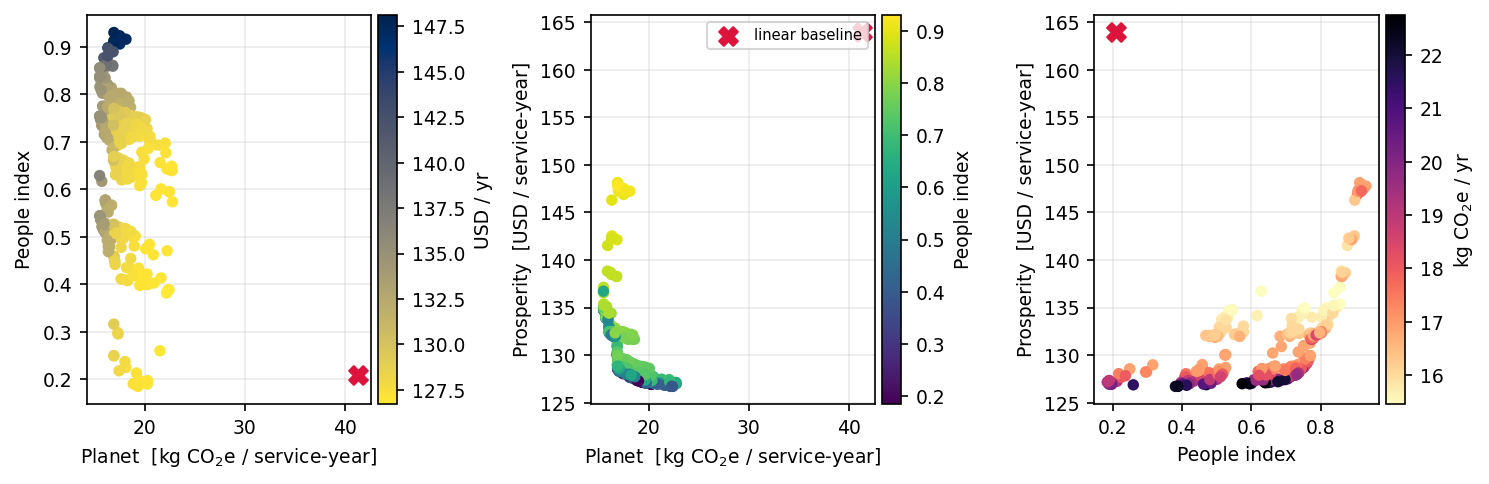
\includegraphics[width=\textwidth]{figures/fig_front.png}
\caption{The Pareto archive in its three pairwise projections; the red cross is
the linear baseline. It sits outside the front on every projection: the
baseline is not a trade-off, it is simply dominated.}
\end{figure}

\begin{figure}[t]
\centering
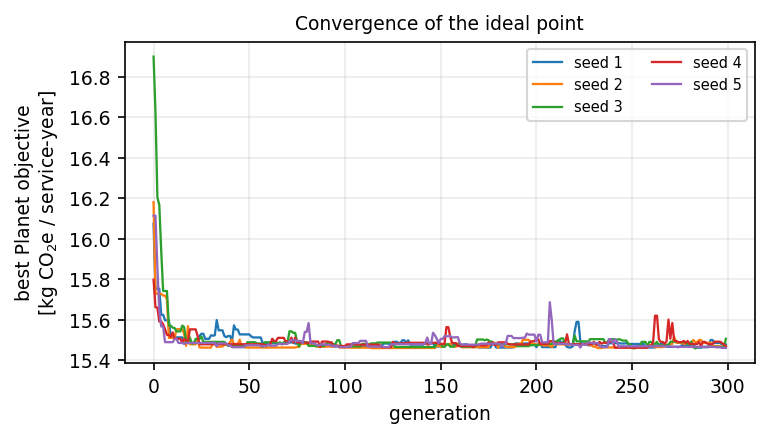
\includegraphics[width=0.62\textwidth]{figures/fig_convergence.png}
\caption{Ideal-point convergence across seeds.}
\end{figure}

\FloatBarrier
\subsection{The central result}

359 of the
359 Pareto designs beat the linear baseline on carbon
\emph{and} cost simultaneously. The best available reduction is
62.6\% on carbon per service-year and
22.7\% on cost per service-year.

Design \#344 is one concrete instance: 100\% recycled polymer, 100\% recycled steel, a 15-year design life with 3 remanufacture cycles, snap-fit/bonded/screwed joints and a 0.3~W standby class. Against the linear baseline it cuts carbon per service-year by 62.6\% and cost per service-year by 16.6\%, while raising the People index by 200\%. It is a top-decile answer in 4\% of the future~$\times$~preference draws.

This is the claim the position statement calls cost-prohibitive, tested rather
than asserted, and the mechanism is not mysterious: circularity in this
product buys its own capital premium back through amortisation. A longer,
remanufacturable life spreads the embodied burden over more service-years, and
the low-standby class pays for itself out of a use phase that dominates the
inventory. The recycled-content lever contributes, but it is the smaller
effect.

\begin{table}[t]
\centering\small
\caption{Corner solutions of the archive, against the linear baseline.
Recycled content is listed polymer/steel/aluminium; joints are enclosure,
chassis, cable entry.}
\begin{tabular}{llllrrrlrrr}
\toprule
& \# & recycled & joints & $L$ & $k$ & sb & EoL & $f_1$ & $f_2$ & People \\
\midrule
linear baseline & -- & 0.00/0.00/0.00 & bond/scre/bond & 8 & 0 & 1.0 & Landfi & 41.34 & 163.91 & 0.210 \\
\midrule
min carbon & \#344 & 1.00/1.00/1.00 & snap/bond/scre & 15 & 3 & 0.3 & Closed & 15.46 & 136.72 & 0.629 \\
min cost & \#80 & 0.43/0.92/0.56 & scre/bond/bond & 15 & 0 & 0.3 & Closed & 22.15 & 126.71 & 0.381 \\
max social & \#198 & 1.00/1.00/1.00 & snap/snap/scre & 8 & 3 & 0.3 & Closed & 16.89 & 147.78 & 0.931 \\
most robust & \#160 & 0.97/1.00/1.00 & snap/snap/scre & 15 & 1 & 0.3 & Closed & 16.06 & 133.22 & 0.820 \\
\bottomrule
\end{tabular}
\end{table}

\begin{figure}[t]
\centering
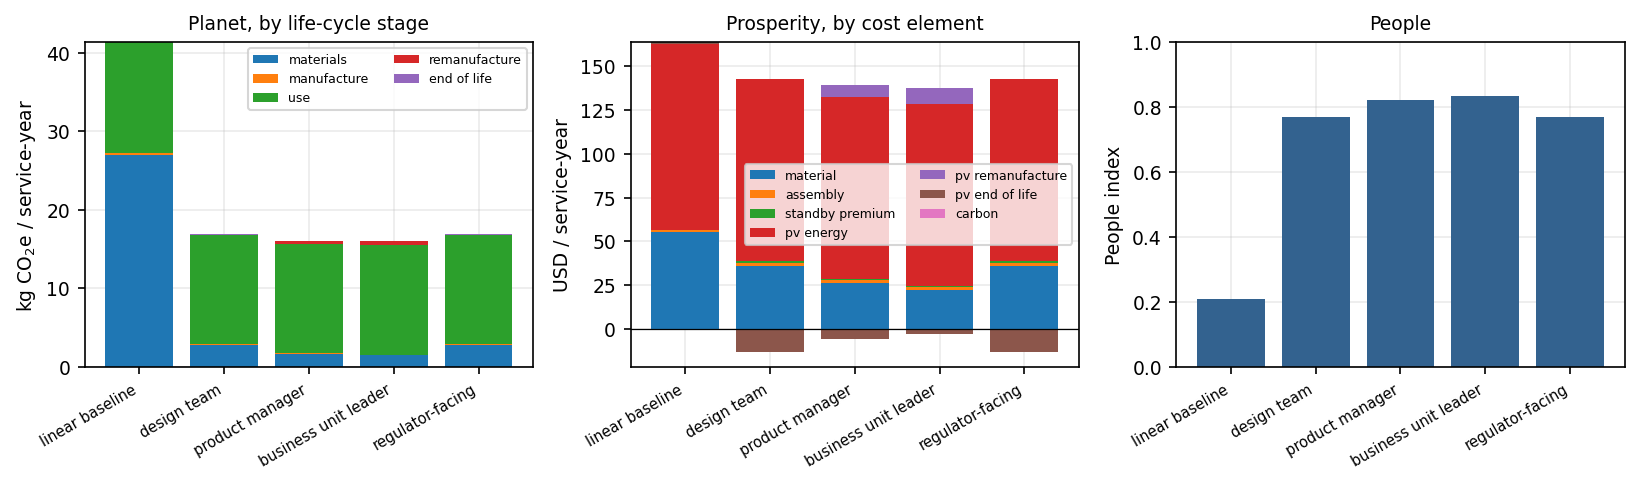
\includegraphics[width=\textwidth]{figures/fig_breakdown.png}
\caption{Where the differences actually come from. Negative cost bars are scrap
revenue recovered at end of life.}
\end{figure}

\FloatBarrier
\subsection{Robustness across futures}

Across 500 futures and
24 preference draws each,
55 of 359 designs clear
twice the chance rate (a design drawn at random would be a top-decile
answer in 10\% of draws, so
20\% is the bar), and 0
are never a top-decile answer at all.
The most robust design, \#160, holds top-decile status in
45\% of draws while remaining feasible in
100\% of futures, including those imposing an ESPR
recycled-content mandate.

The mechanism behind robustness is worth naming, because it is a design
instruction rather than a number. Designs that survive share reversible
joints, a long design life and meaningful recycled content. Those are exactly
the choices that hedge: reversible joints keep the remanufacturing option open
if labour economics improve, recycled content keeps the design compliant if a
delegated act lands, and a long life dilutes embodied carbon regardless of how
fast the grid decarbonises. Robustness here is not a statistical artefact, it
is optionality.

\begin{figure}[t]
\centering
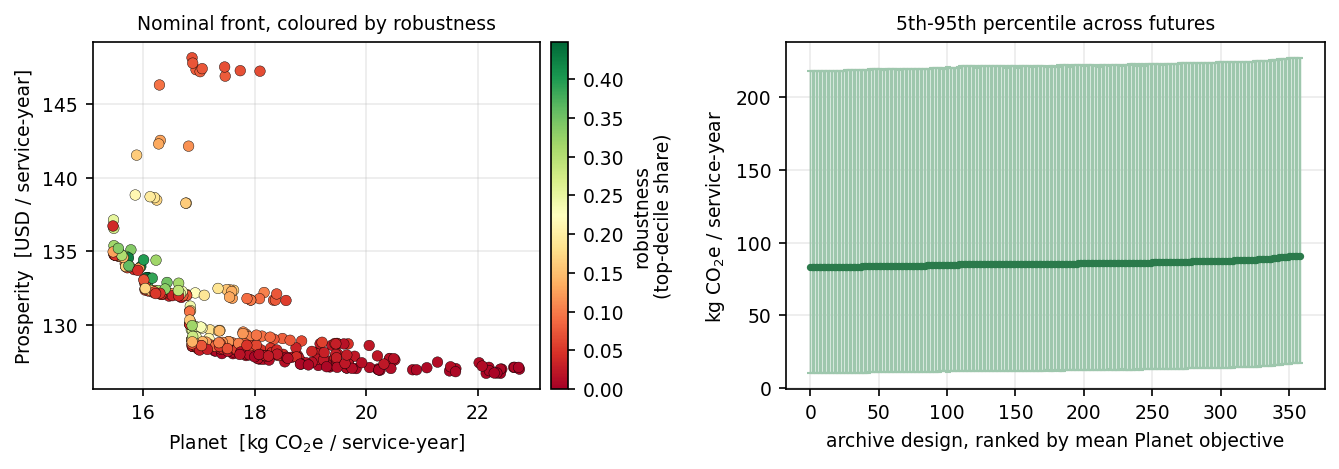
\includegraphics[width=\textwidth]{figures/fig_robustness.png}
\caption{Left: the nominal front coloured by robustness: note that the
cheapest nominal designs are not the most robust. Right: 5th--95th percentile
spread of the Planet objective across futures, which is dominated by grid
decarbonisation and charging-throughput uncertainty.}
\end{figure}

\FloatBarrier
\subsection{The decision aid}
\label{sec:aid}

\begin{table}[h]
\centering\small
\caption{What each profile selects. Weights are (Planet, Prosperity, People);
$f_1$ and $f_2$ are means across the ensemble.}
\begin{tabular}{llllrlrrrrr}
\toprule
profile & weights & pick & share & winners & recycled & $L$ & $k$ & sb & $\bar f_1$ & $\bar f_2$ \\
\midrule
design team & 0.45/0.15/0.40 & \#346 & 12\% & 61 & 1.00/1.00/1.00 & 15 & 0 & 0.3 & 85.09 & 150.53 \\
product manager & 0.20/0.55/0.25 & \#160 & 33\% & 18 & 0.97/1.00/1.00 & 15 & 1 & 0.3 & 83.96 & 154.93 \\
business unit leader & 0.30/0.50/0.20 & \#351 & 31\% & 20 & 1.00/0.97/0.94 & 15 & 2 & 0.3 & 83.78 & 157.47 \\
regulator-facing & 0.55/0.20/0.25 & \#346 & 69\% & 39 & 1.00/1.00/1.00 & 15 & 0 & 0.3 & 85.09 & 150.53 \\
\bottomrule
\end{tabular}
\end{table}

Four profiles produce 3 distinct recommendations from one
front. No profile's choice wins in every future: the shares in the table
are the honest answer to ``what should we build?'', and their distance from
100\% is the residual uncertainty a committee, not an optimiser, has to
absorb.

\begin{figure}[t]
\centering
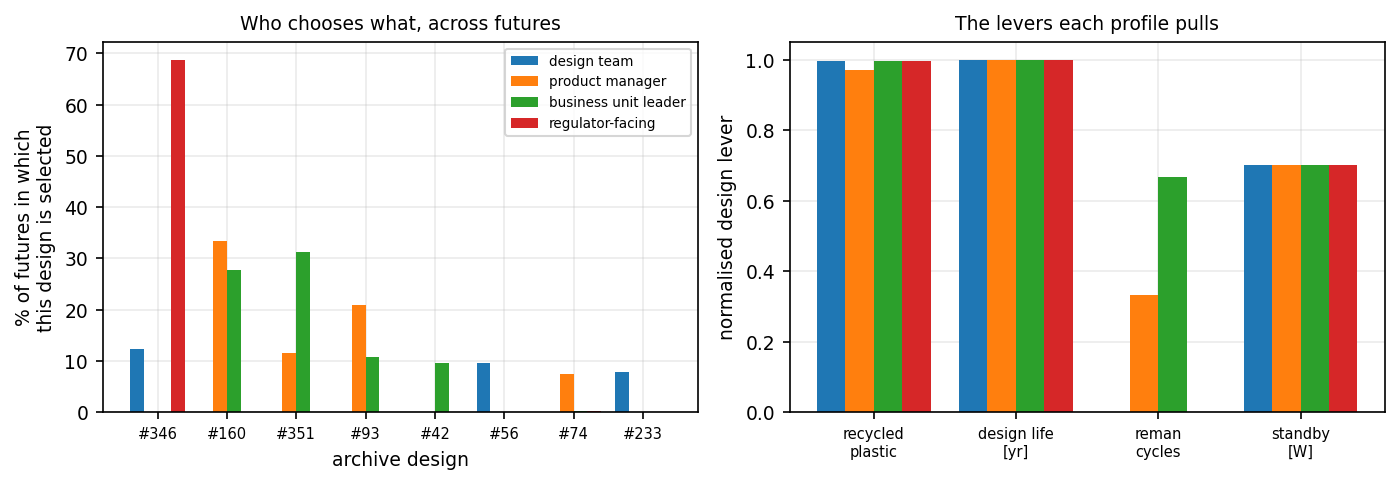
\includegraphics[width=\textwidth]{figures/fig_profiles.png}
\caption{Left: how often each archive design is selected, by profile. Right:
the levers each profile's modal choice pulls, normalised.}
\end{figure}

\FloatBarrier
\FloatBarrier
\section{Testing the choices that could decide the answer}

A life-cycle model contains a small number of choices that are not measurements
and that can move the conclusion more than any design variable. Declaring them
is necessary; testing them is what makes the study checkable. Six are tested
here, and two of the six change the answer.

\subsection{Impact category: was optimising carbon a fair proxy?}

The inventory carries four indicators. Ranking the whole archive under each and
correlating against global warming gives Table~\ref{tab:indrank}.

\begin{table}[h]
\centering\small
\caption{Rank agreement with global warming across the 359-design archive.}
\label{tab:indrank}
\begin{tabular}{lrrc}
\toprule
indicator & Spearman $\rho$ & Kendall $\tau$ & picks the same best design \\
\midrule
cumulative energy demand (MJ) & +0.971 & +0.894 & NO \\
EF 3.1 single score (Pt) & +0.929 & +0.875 & yes \\
EF 3.1 resource use, minerals and metals (Pt) & +0.921 & +0.859 & yes \\
\bottomrule
\end{tabular}
\end{table}

Agreement is high but not perfect. Carbon is a defensible proxy for ranking
designs in this product, and it is not a substitute for the other indicators
when selecting a single winner. Reporting the correlation is the honest form of
that statement; reporting only the carbon front and calling it an LCA would not
have been.

\subsection{Allocation: the choice that does decide the answer}

ISO 14044 requires the allocation convention to be declared and its influence
examined. Under \emph{cut-off}, recovered material earns nothing and
end-of-life is 0.32\,\% of total carbon, a rounding error, which
makes the end-of-life decision variable environmentally inert. Under
\emph{substitution} it earns the virgin production it displaces and rises to
14.9\,\% of the total, shifting the mean Planet objective by
-13.2\,\%.

The consequence is larger than the shift. Rank correlation between the two
conventions across the archive is $\rho=+0.666$, and they do not agree on
the best design. \textbf{The allocation convention, not the design space,
selects the winner.} Any result in this report that concerns end-of-life route
is conditional on the convention stated with it. This is the single most
important methodological caveat in the study, and it is why the earlier
carbon-reporting-factor version of this model (which had no substitution
option at all) could not have been trusted on circularity questions.

Rather than stop at two independently invented conventions, a third is
implemented: the material term of the European Commission's own \emph{Circular
Footprint Formula} (CFF), the method the Product Environmental Footprint
regulation actually specifies for exactly this problem [13]:
\[
E = (1-R_1)E_V + R_1\left[A\,E_{\text{recycled}}
+ (1-A)E_V\frac{Q_{s,\text{in}}}{Q_p}\right],
\]
where $R_1$ is the recycled-content decision variable already in this model,
$E_V$ and $E_{\text{recycled}}$ the virgin and secondary production
processes, and $A\in[0,1]$ a market-based allocation factor splitting the
benefit of recycling between the material's two lives. At $A=1$ the formula
collapses exactly onto this model's \emph{substitution} convention on both the
input side and end-of-life -- confirmed numerically as a correctness check,
not asserted -- and at $A=0$ recycled content earns almost no credit. Sweeping
$A\in\{0,\,0.5,\,1\}$ moves the archive's mean Planet objective by
60.0\,\% across the sweep, and CFF's rank correlation against the
existing conventions is $\rho=+0.871$ (cut-off) and
$\rho=+0.665$ (substitution) -- a third, citable point inside the same
disagreement, not outside it.

Two things are stated plainly about this implementation rather than left for
a reader to discover. First, $A=0.5$ is the commonly cited PEF default for
market-based allocation, not a value verified here for aluminium, steel,
copper or plastic specifically -- it is swept as a sensitivity, not asserted
as this product's true factor. Second, the CFF's material formula is
implemented; its energy-recovery and disposal formula components (parameters
$B$, calorific value and recovery efficiencies) could not be verified against
a primary EU/JRC source at the time of writing -- several official PDF
documents returned access errors during research for this feature -- and
guessing a regulatory formula would be a worse error than not implementing
it. End-of-life under \texttt{cff} therefore falls back to this model's own
\emph{substitution} treatment, labelled in code as an approximation, not a
citation. Partial coverage, verified precisely, was judged better than full
coverage, guessed.

\subsection{Geography: the level moves, the ranking does not}

\begin{table}[h]
\centering\small
\caption{Grid sensitivity. Mean Planet objective across the archive, by market.}
\label{tab:geo}
\begin{tabular}{lrrr}
\toprule
grid & \si{\kilo\gram} CO$_2$e/kWh & mean Planet & $\rho$ vs reference \\
\midrule
Sweden (reference) & 0.0413 & 17.7 & -- \\
France & 0.0438 & 18.6 & +1.000 \\
EU-27 & 0.2370 & 84.1 & +0.998 \\
Netherlands & 0.3284 & 115.1 & +0.997 \\
Germany & 0.3407 & 119.3 & +0.996 \\
Poland & 0.6363 & 219.6 & +0.987 \\
\bottomrule
\end{tabular}
\end{table}

The absolute result spans 12$\times$ between the cleanest and dirtiest
European grid: larger than the effect of every design variable combined. But
rank correlation across the archive stays above $+0.99$ everywhere. So the
level of the answer is a statement about the grid, while the \emph{ranking} of
designs is not. A designer can use this front anywhere in Europe; a
communications department quoting the absolute number cannot.

\subsection{The recyclate constants: a finding with its conditionality attached}

Three constants govern the cost penalty on recycled content: a quality
threshold, a quadratic surcharge and a reject rate. \textbf{None has an
empirical source.} They matter because they produce the interior cost optimum
in recycled content, i.e.\ the result that recycled content is not simply
maximised.

Sweeping all three over their plausible ranges: the interior optimum exists in
22 of 27 of the corner combinations tested, but its location moves between
0.43 and 1.00 recycled content. The honest statement is
therefore narrow: \emph{that} an interior optimum exists is reasonably robust to
these constants; \emph{where} it sits is not, and no number quoted from this
model for an optimal recycled content should be read as an empirical estimate.
Measuring these three constants for a real recyclate stream would be the single
most valuable piece of primary data this model could receive.

\subsection{Social weights: a property of the designs, mostly}

The four social sub-weights were chosen, not elicited. Redrawing them
400 times from a flat Dirichlet, the nominally best design remains best
in 100\,\% of draws, with 1 distinct winners overall, and
rank correlation against the nominal weighting averages $\rho=+0.940$
(5th percentile $+0.782$). The social ranking is therefore mostly a property
of the designs rather than of the weighting, but the 1 distinct
winners are a reminder that this index is a transparent decision aid, not a
measurement.

\subsection{Scenario widths: not load-bearing}

\begin{table}[h]
\centering\small
\caption{Robustness ranking under halved and doubled judgement widths.
Measured widths (commodity volatility) and the discrete grid set are unchanged.}
\begin{tabular}{lrrr}
\toprule
judgement $\sigma$ & top design & robust core & $\rho$ vs nominal \\
\midrule
$\times$0.5 & \#160 & 54 & +0.999 \\
$\times$1.0 & \#160 & 53 & +1.000 \\
$\times$2.0 & \#160 & 54 & +0.998 \\
\bottomrule
\end{tabular}
\end{table}

A factor of four in the guessed widths leaves the top design unchanged and rank
correlation above $+0.98$. The robustness conclusions do not rest on the
distribution widths.

\subsection{Electronics: how wrong would the weakest proxy have to be?}

Electronics has no matching Idemat process at all -- no entry represents a
charging-station metering or RCD board. Rather than pin one white-goods
control board arbitrarily, the factor used here is the average of the two
closest analogues, a refrigerator and a washing-machine control board
(\texttt{data/idemat\_process\_map.json}
\allowbreak\texttt{-> families.electronics.virgin}), following the same
"use the available evidence rather than one arbitrary pick" logic as the
aluminium choice. Both source processes explicitly exclude integrated
circuits, a real limitation the averaging does not resolve.

At today's factor, aluminium accounts for 82\,\% of material-stage
carbon and electronics 10\,\%. Electronics would have to be roughly 8.3x its current factor before it overtakes aluminium as the largest material contributor -- a far larger error than the scenario ensemble's own perturbation of this factor. Across the tested range the archive's ranking barely moves regardless (worst-case Spearman +0.933) because electronics mass is not a decision variable -- scaling its factor shifts every design's score together.
This is a stronger statement than a wide error bar: it says exactly how wrong
the proxy would have to be before it changed which material dominates the
carbon story, rather than asserting robustness by perturbing it and hoping.

\subsection{Prices: USGS against a second, independent source}

USGS never resolved an aluminium price -- the download was blocked at
data-collection time -- so aluminium ran on a hardcoded guess
(\SI{2.55}{} USD/kg) until this fix. It now uses the World Bank Commodity
Markets ("Pink Sheet") trailing 12-month mean instead, a live, independently
compiled global reference series: \SI{3.10}{} USD/kg against the
guess it replaces. For copper, where USGS does have data, the two sources are
compared directly: USGS \SI{9.48}{} versus World Bank
\SI{12.09}{} USD/kg, a +0.15\,\% shift in mean archive
cost between sources, rank correlation $\rho=+1.000$, same best design:
yes. Steel has no comparable World Bank entry -- that source
publishes iron ore, not scrap, a different commodity -- so this cross-check
covers aluminium and copper only, and that limitation is stated rather than
papered over with an approximate substitute.

\subsection{Does the design decision matter more than the modelling decision?}

Every methodological sensitivity in this section can be put on one axis: how
much does each one move the Planet objective, compared to moving across the
entire 359-design Pareto archive itself?

\begin{table}[h]
\centering\small
\caption{Spread in the Planet objective, \si{\kilo\gram} CO$_2$e per
service-year, induced by each choice, design space held fixed except where
the choice itself is the design archive.}
\label{tab:spread}
\begin{tabular}{lr}
\toprule
source of variation & span \\
\midrule
grid region (6 European markets) & 201.9 \\\\
inventory backend (Idemat vs DEFRA) & 57.8 \\\\
design choice (whole Pareto archive) & 7.3 \\\\
allocation convention (cut-off vs substitution) & 2.3 \\\\
\bottomrule
\end{tabular}
\end{table}

Design choice ranks \#3 of 4 by how much it moves the
result. 2 purely methodological choices move the Planet objective more than the entire design space does. That is not a reason to stop optimising the
design -- the win-win designs this report finds are real and reproducible --
but it is a reason to report the modelling choices with the same weight as the
design recommendation, which is what Sections~7 and~9 of this report do rather
than treating them as footnotes to it.

\FloatBarrier
\section{Does the optimiser earn its keep?}

Earlier versions of this work reported that random search reached a large
fraction of NSGA-III's hypervolume, without testing whether the difference was
real. It is now tested properly: 10 independent seeds per method, an
identical evaluation budget of 11\,132 per run, and the same variation
operators for both evolutionary algorithms so the comparison isolates the
selection mechanism.

\begin{table}[h]
\centering\small
\caption{Hypervolume by method, over 10 seeds each.}
\begin{tabular}{lrrrr}
\toprule
method & seeds & median & mean & s.d. \\
\midrule
NSGA-III & 10 & 204.27 & 204.03 & 1.20 \\
NSGA-II & 10 & 206.61 & 206.59 & 0.32 \\
random search & 10 & 185.78 & 185.93 & 1.87 \\
\bottomrule
\end{tabular}
\end{table}

\begin{table}[h]
\centering\small
\caption{Pairwise Mann--Whitney $U$, two-sided, with rank-biserial effect
size, following the nonparametric evolutionary-algorithm comparison protocol
of [21]. With ten seeds per method the test is weakly powered, so the effect
size carries more information than the $p$-value and both are reported.}
\begin{tabular}{lrrrrc}
\toprule
comparison & median ratio & $U$ & $p$ & effect $r$ & $p<0.05$ \\
\midrule
NSGA-III vs NSGA-II & 0.9887 & 0 & 0.0002 & 1.00 & yes \\
NSGA-III vs random search & 1.0996 & 0 & 0.0002 & 1.00 & yes \\
NSGA-II vs random search & 1.1122 & 0 & 0.0002 & 1.00 & yes \\
\bottomrule
\end{tabular}
\end{table}

Both evolutionary algorithms beat random search by roughly 10\,\% in
median hypervolume [20], with complete rank separation across ten seeds.

The comparison between them is less comfortable, and is reported as it came
out. \textbf{NSGA-II attains a 1.1\,\% higher median hypervolume
than NSGA-III, and the separation is complete} ($U=0$, $r=1.00$,
$p=0.00016$): every NSGA-II seed beat every NSGA-III seed. The margin is small
in absolute terms and both algorithms sit far above random search, but the
direction is consistent and the test is unambiguous, so the honest statement is
that \emph{NSGA-III is not the better optimiser on this problem}.

That is what should be expected, and saying so is more useful than explaining
it away. Reference-point niching is designed for many-objective problems where
crowding distance degrades; with three objectives, crowding distance is still a
perfectly good diversity signal, and NSGA-III's uniform reference lattice
spends population on regions of the simplex that this front does not occupy.

NSGA-III is nonetheless what the rest of this report uses, for a reason that is
not performance: its reference directions are where decision-maker preferences
attach, which is the mechanism Section~\ref{sec:aid} depends on. A reader who
wants the best-converged front on this problem should use NSGA-II; a reader who
wants the decision aid should use NSGA-III and accept 1.1\,\% of
hypervolume as its price. Both are implemented, share the same variation
operators, and can be swapped with one argument.

\FloatBarrier
\section{Where the validation gap actually comes from}

Section~\ref{sec:validation} reported the aggregate agreement with the
published study. Aggregates hide whether agreement is accuracy or cancellation,
so the difference is decomposed by material family in
Table~\ref{tab:vdecomp}.

\begin{table}[h]
\centering\small
\caption{Contribution of each family to the difference against the published
study, \si{\kilo\gram} CO$_2$e per unit.}
\label{tab:vdecomp}
\begin{tabular}{lrrrr}
\toprule
family & mass (kg) & model factor & published factor & contribution \\
\midrule
aluminium & 14.61 & 11.751 & 13.056 & -19.1 \\
electronics & 4.30 & 4.853 & -- & -- \\
plastic & 2.72 & 2.690 & 3.310 & -1.7 \\
steel & 1.72 & 2.509 & 1.727 & +1.3 \\
copper & 1.15 & 3.451 & 3.560 & -0.1 \\
\bottomrule
\end{tabular}
\end{table}

The gap is not spread across the inventory: 86\,\% of what remains of
it is the aluminium factor alone, and only 12\,\% of the
family-level disagreement cancels in the total. That is a better outcome than
broad agreement would have been, because it is attributable.

The attribution is a supply-chain geography choice, and it was made the right
way round: on evidence, before checking the fit, not after. Idemat resolves
both a global-average primary aluminium route and a European one. GARO's own
LCA report names no smelter, grid, or bauxite origin for the aluminium in the
LS4, but its own supplier transport-distance table lists routes to Gnosjö
from Poland, Germany, the Czech Republic, Italy, Turkey, China, Denmark and
Slovenia, describing a genuinely international supplier base, not a
predominantly Nordic one. On that evidence this report defaults to the
\emph{global} route (\SI{11.75}{\kilo\gram} CO$_2$e/kg), and keeps
the European route (\SI{4.81}{\kilo\gram} CO$_2$e/kg, hydro- and
nuclear-heavy smelting) only as a labelled comparison.

That choice happens to move the model closer to the published study's own
factor (\SI{13.06}{\kilo\gram} CO$_2$e/kg): the default gives a
cradle-to-gate ratio of 0.66 against the published figure, where
substituting the European alternative would give 0.34, \emph{further}
from the published result, not closer. That agreement is worth stating plainly
as a consequence, not a justification: the route was chosen on the transport
evidence first, and only checked against the published figure afterwards. Had
the two disagreed, the transport evidence would still have been the better
basis for the default.

Neither study is wrong on this point; they simply required different evidence
to resolve, and only one source (GARO's own transport data) actually bears on
which is closer to this product's real supply chain. For a product that is
60\,\% aluminium by mass, that one declared, evidenced choice is
worth more than every circular design decision in this report combined,
which is itself the most useful thing the validation exercise produced.

What remains of the gap after that reconciliation (0.66 of the
published figure) should not be chased further by tuning; the more defensible
move is to size it against what independent LCA studies find when they compare
databases for the \emph{same} product. Pauer, Wohner and Tacker modelled six
packaging systems in three database/software combinations (GaBi, ecoinvent
3.6, and the EU's own EF database) and found that while global-warming results
were broadly similar across databases, other impact categories diverged
substantially, driven by differences in background-process scope and
characterisation coverage between databases [14]. A companion
study of LCI database choice in a drivetrain (combustion vs. electric vehicle)
case study reports ecoinvent-vs-GaBi deviations from 15\,\% up to several
thousand per cent depending on the impact category [15].
Against that published range, a residual gap of
this size between two independently built inventories applied to the same
product is the expected order of magnitude, not evidence of an error in
either.

\section{What this model cannot tell you}

Several limitations of earlier versions of this work have been closed and are
recorded here as closed rather than quietly dropped: the inventory is now
process-level and multi-indicator rather than a single carbon-reporting factor;
the end-of-life credit convention is implemented three ways, including the
EU's own regulatory formula, and tested rather than fixed by the dataset's
convention; the circularity indicator follows the published formula rather
than a simplification; the scenario widths for commodity prices are measured
rather than guessed; the electronics proxy is an average across the available
evidence with a quantified breakeven bound rather than one arbitrary pick;
aluminium pricing comes from a live independent source rather than a
hardcoded guess; and the aluminium production route was chosen from evidence
in the product's own published transport data, before checking whether it
improved agreement with anything, not after. What remains is below.

\begin{itemize}
\item \textbf{The allocation convention selects the winner.} This is the
binding limitation, not a footnote. Cut-off and substitution rank the archive
almost independently ($\rho=+0.666$) and disagree on the best design. Any
end-of-life conclusion here is conditional on the convention quoted beside it,
and a reader who needs one answer rather than two must decide the convention
on grounds this model cannot supply.
\item \textbf{The material masses are cited; their allocation to components
is not.} The published study gives mass by material, not by part. Anything
depending only on how much aluminium or electronics the product contains is on
cited ground; anything depending on \emph{which part} the aluminium is in
(disassembly sequence above all) rests on this project's allocation. The
repairability term is the most exposed.
\item \textbf{The recyclate constants are unmeasured, and they set the
optimum's location.} The interior optimum exists across most of the parameter
space, but sits anywhere between 0.43 and 1.00 recycled
content. No optimal recycled content quoted from this model is an empirical
estimate.
\item \textbf{The electronics process is a stand-in, bounded rather than
merely disclosed.} The average of two white-goods control boards represents
the metering, RCD and power boards; both source processes exclude integrated
circuits. It remains the weakest mapping in the inventory. What changed is
that the weakness is now bounded rather than only flagged: Section 8.1 shows
electronics would need to be wrong by more than 8.3x its factor
before it changed which material dominates the carbon story, and the
archive's ranking barely moves across that range regardless, because
electronics mass is not itself a decision variable.
\item \textbf{The People index is a proxy, not a social LCA.} It is a
transparent weighted index over four design-controllable indicators. It is not
a UNEP S-LCA study [26]: there is no stakeholder inventory, no worker or
community subcategory, and no site-specific data. The Dirichlet re-weighting shows the
ranking is not an artifact of the weights; it cannot validate the choice of
terms, and no claim about actual social performance follows from it.
\item \textbf{One inventory, no uncertainty data.} Idemat publishes point
values, not distributions. The proxy multipliers in the ensemble are a stand-in
for inventory uncertainty, not a propagation of it. A study with access to
ecoinvent's uncertainty information could do this properly.
\item \textbf{Prices are world-market, impacts are European.} USGS and World
Bank both quote globally traded metals, which is defensible for commodities
(Section 8.2 shows the two sources agree to within +0.15\,\% on
archive cost and pick the same best design), but this leaves polymer and
labour prices as assumptions rather than data, and steel has no comparable
World Bank series to cross-check against at all.
\item \textbf{The CFF's disposal formula is not implemented.} Only the
material (input-side) term of the EU PEF Circular Footprint Formula is
implemented; its energy-recovery and disposal terms could not be verified
against a primary EU/JRC source and are not guessed. End-of-life under the
\texttt{cff} convention falls back to this model's own substitution
treatment as a stated approximation, not a citation.
\item \textbf{Nothing here is validated against measurement.} The one
external check is against another model. Agreement between two models is
weaker evidence than either being right, and the residual gap after
reconciling the aluminium route is sized against the published range of
inter-database LCA discrepancies rather than closed further by tuning.
\end{itemize}

The central finding (that carbon-and-cost win-win designs exist and can be
found systematically) is a statement about the \emph{structure} of the
trade-off, and it survives every perturbation tested: all four impact
categories, three allocation conventions including the EU's own CFF, six
European grids, two independent price sources, an order-of-magnitude range in
the electronics factor, a factor of four in the scenario widths, and random
re-weighting of the social index. What does \emph{not} survive unqualified is
the implicit assumption that design choice is the largest lever available:
Section 8.3 finds it usually is not. The specific numbers should not be
carried past the limitations above.

\section{Appendix: the declared assumptions}

Every quantity below is an engineering estimate rather than a dataset value.
They are collected in one class in \texttt{circuopt/model.py} so that a
reviewer can replace any of them without touching the model.

\begin{table}[h]
\centering\small
\begin{tabular}{lrlp{6.4cm}}
\toprule
parameter & value & unit & what it represents \\
\midrule
\texttt{mfg\_energy\_kwh\_per\_kg} & 2.4 & kWh/kg & assembly energy intensity \\
\texttt{energy\_delivered\_kwh\_per\_year} & 33333.3 & kWh/yr & charging throughput \\
\texttt{conversion\_loss\_frac} & 0.01 & -- & AC station switching losses \\
\texttt{reman\_life\_extension} & 0.666667 & -- & service-life gain per remanufacture cycle \\
\texttt{reman\_part\_replacement\_frac} & 0.18 & -- & mass renewed per cycle \\
\texttt{labour\_rate\_usd\_per\_hour} & 34 & USD/h & loaded EU manufacturing rate \\
\texttt{plastic\_virgin\_usd\_per\_kg} & 2.4 & USD/kg & PC/ABS resin, no open index available \\
\texttt{electronics\_usd\_per\_kg} & 68 & USD/kg & populated PCBA and contactor \\
\texttt{electricity\_price\_usd\_per\_kwh} & 0.31 & USD/kWh & EU household tariff \\
\texttt{scrap\_recovery\_efficiency} & 0.85 & -- & closed-loop yield \\
\texttt{collection\_cost\_usd\_per\_kg} & 0.35 & USD/kg & WEEE take-back logistics \\
\texttt{discount\_rate} & 0.05 & -- & life-cycle costing \\
\texttt{repair\_time\_target\_s} & 300 & s & EN 45554-style disassembly benchmark \\
\texttt{recyclate\_threshold} & 0.4 & -- & recycled content below which there is no quality penalty \\
\texttt{recyclate\_cost\_penalty} & 0.6 & -- & quadratic surcharge coefficient $\lambda$ \\
\texttt{recyclate\_reject\_rate} & 0.09 & -- & extra input mass per kilogram of good part at $r=1$ \\
\bottomrule
\end{tabular}
\end{table}

\FloatBarrier
\section{Reproducing this}

\begin{verbatim}
python3 circuopt/datasets.py      # parse and cache the two open datasets
python3 test_circuopt.py          # regression suite
python3 scripts/fetch_idemat.py   # one-time: Idemat 2026 (free, attribution)
python3 scripts/fetch_worldbank.py # one-time: World Bank commodity prices
python3 run_experiments.py        # E0-E15, writes results.json + figures/
python3 make_report.py            # regenerates this PDF from results.json
\end{verbatim}

Requires Python 3.8+, NumPy, Matplotlib and \texttt{openpyxl} (to read the
DEFRA workbook). Total runtime for the full protocol was
\SI{7487}{\second} on one core. The raw datasets are
included under \texttt{data/} under the terms of their respective licences.

\section*{Data and licences}
\small
\begin{itemize}
\item Idemat 2026, Sustainability Impact Metrics / Delft University of
Technology. Free to use with attribution; fetched by
\texttt{scripts/fetch\_idemat.py}, not redistributed with this repository.
\item UK Government GHG Conversion Factors for Company Reporting 2025,
Department for Energy Security and Net Zero. Open Government Licence v3.0.
Retained as a second, independent inventory backend for comparison.
\item Mineral Commodity Summaries 2025 salient-statistics data releases,
U.S. Geological Survey. Public domain (17 U.S.C. \S 105).
\item Commodity Markets ("Pink Sheet") monthly price data, World Bank.
Freely available World Bank data; fetched by
\texttt{scripts/fetch\_worldbank.py}, not redistributed. Used as the live
source for aluminium pricing (USGS never resolved this commodity) and as a
second, independent price source for copper.
\item GARO LS4 Life Cycle Assessment, Persson \& Erselius (GARO AB / 2050
Consulting), July 2021. Published manufacturer report, cited throughout for
the product's bill of materials and service life.
\end{itemize}

\section*{References}
\small
\begin{enumerate}[label={[\arabic*]}]
\item J. Persson and G. Erselius, \emph{Life Cycle Assessment of the charging
station GARO LS4}, GARO AB with 2050 Consulting, July 2021. Available from
GARO AB; a copy is included at \texttt{data/garo\_ls4\_lca.pdf}.
\item J.G. Vogtlander, \emph{Idemat 2026}, Sustainability Impact Metrics /
Delft University of Technology, \texttt{ecocostsvalue.com}. Free to use with
attribution; not redistributed with this repository.
\item European Commission, \emph{Environmental Footprint (EF) 3.1 reference
package}, Joint Research Centre.
\item ISO 14044:2006, \emph{Environmental management: Life cycle assessment,
requirements and guidelines}, clause 4.3.4 on allocation.
\item H.B. Mann and D.R. Whitney, ``On a test of whether one of two random
variables is stochastically larger than the other,'' \emph{Annals of
Mathematical Statistics}, 18(1), 50--60, 1947.
\item K. Deb and H. Jain, ``An evolutionary many-objective optimization
algorithm using reference-point-based nondominated sorting approach, part I,''
\emph{IEEE Trans. Evolutionary Computation}, 18(4), 577--601, 2014.
\item K. Deb, A. Pratap, S. Agarwal, T. Meyarivan, ``A fast and elitist
multiobjective genetic algorithm: NSGA-II,'' \emph{IEEE Trans. Evolutionary
Computation}, 6(2), 182--197, 2002.
\item I. Das and J. E. Dennis, ``Normal-boundary intersection,''
\emph{SIAM J. Optimization}, 8(3), 631--657, 1998.
\item A. P. Wierzbicki, ``The use of reference objectives in multiobjective
optimization,'' in \emph{Multiple Criteria Decision Making Theory and
Application}, Springer, 1980.
\item Ellen MacArthur Foundation and Granta Design, \emph{Circularity
Indicators: An Approach to Measuring Circularity, Methodology}, 2015. The
MCI in this report follows this formulation, including $F(X)=0.9/X$.
\item Regulation (EU) 2024/1781 establishing a framework for the setting of
ecodesign requirements for sustainable products (ESPR).
\item EN 45554:2020, General methods for the assessment of the ability to
repair, reuse and upgrade energy-related products.
\item European Commission, Joint Research Centre, \emph{Product
Environmental Footprint Category Rules (PEFCR) Guidance}, which defines the
Circular Footprint Formula. The primary document could not be fetched
directly during this work (access was blocked); the formula implemented here
was reconstructed from secondary summaries of the guidance (GreenDelta,
2020; ARECO) and should be checked against the primary JRC document before
being relied on beyond this report.
\item E. Pauer, B. Wohner, M. Tacker, ``The Influence of Database Selection
on Environmental Impact Results. Life Cycle Assessment of Packaging Using
GaBi, Ecoinvent 3.6, and the Environmental Footprint Database,''
\emph{Sustainability}, 12(23), 9948, 2020.
\href{https://doi.org/10.3390/su12239948}{doi:10.3390/su12239948}.
\item M. Kalverkamp, E. Helmers, A. Pehlken, ``Impacts of life cycle
inventory databases on life cycle assessments: A review by means of a
drivetrain case study,'' \emph{Journal of Cleaner Production}, 269, 121329,
2020. \href{https://doi.org/10.1016/j.jclepro.2020.121329}{doi:10.1016/j.jclepro.2020.121329}.
\item N. Srinivas and K. Deb, ``Multiobjective Optimization Using
Nondominated Sorting in Genetic Algorithms,'' \emph{Evolutionary
Computation}, 2(3), 221--248, 1994. The original NSGA, the direct ancestor
of NSGA-II and NSGA-III.
\item K. Deb and R.B. Agrawal, ``Simulated Binary Crossover for Continuous
Search Space,'' \emph{Complex Systems}, 9, 115--148, 1995. The crossover
operator used on the continuous genes throughout this work.
\item K. Deb and M. Goyal, ``A Combined Genetic Adaptive Search (GeneAS) for
Engineering Design,'' \emph{Computer Science and Informatics}, 26(4),
30--45, 1996. Introduces the polynomial mutation operator used alongside SBX.
\item H. Jain and K. Deb, ``An Evolutionary Many-Objective Optimization
Algorithm Using Reference-Point-Based Nondominated Sorting Approach, Part II:
Handling Constraints and Extending to an Adaptive Approach,'' \emph{IEEE
Trans. Evolutionary Computation}, 18(4), 602--622, 2014. Extends NSGA-III to
constrained problems, which is the form implemented here.
\item E. Zitzler and L. Thiele, ``Multiobjective Optimization Using
Evolutionary Algorithms: A Comparative Case Study,'' in \emph{Parallel
Problem Solving from Nature: PPSN V}, Springer, 292--301, 1998.
Introduces the hypervolume indicator used throughout Section~8 to compare
NSGA-III, NSGA-II and random search.
\item J. Derrac, S. Garc\'ia, D. Molina, F. Herrera, ``A Practical Tutorial
on the Use of Nonparametric Statistical Tests as a Methodology for Comparing
Evolutionary and Swarm Intelligence Algorithms,'' \emph{Swarm and
Evolutionary Computation}, 1, 3--18, 2011. Basis for the Mann--Whitney
protocol and the emphasis on effect size over $p$-value with small seed
counts.
\item W. Kl\"opffer, ``Life Cycle Sustainability Assessment of Products,''
\emph{International Journal of Life Cycle Assessment}, 13(2), 89--95, 2008.
The LCA + LCC + S-LCA framing this report's three objectives instantiate.
\item T.E. Swarr, D. Hunkeler, W. Kl\"opffer et al., ``Environmental
Life-Cycle Costing: A Code of Practice,'' \emph{International Journal of
Life Cycle Assessment}, 16, 389--391, 2011. The LCC methodology the
Prosperity objective follows.
\item J. Kirchherr, D. Reike, M. Hekkert, ``Conceptualizing the Circular
Economy: An Analysis of 114 Definitions,'' \emph{Resources, Conservation and
Recycling}, 127, 221--232, 2017. Notes that most circular-economy
definitions barely connect to social equity, which is part of the motivation
for treating People as a full, independent objective rather than a
constraint.
\item D. Figueirinhas, Y. Vakulenko, H. P\r{a}lsson, D. Hellstr\"om,
``Advancing Circularity Metrics: Revisiting the Ellen MacArthur Foundation's
Material Circularity Indicator,'' \emph{Resources, Conservation and
Recycling}, 226, 108682, 2025. Documents specific methodological weaknesses
in the MCI formula this report also implements (most relevantly its
single-cycle view and its treatment of the 50:50 waste-allocation split),
and is why the MCI values reported here are labelled against the published
formula rather than presented as a fully resolved circularity measure.
\item United Nations Environment Programme, \emph{Guidelines for Social Life
Cycle Assessment of Products and Organisations 2020}, UNEP/SETAC Life Cycle
Initiative, 2020. The methodology the People index explicitly does not
implement; cited so the distinction in Section~10 is checkable.
\item Directive 2012/19/EU of the European Parliament and of the Council of
4 July 2012 on waste electrical and electronic equipment (WEEE) (recast).
Basis for treating end-of-life collection and recovery as a first-class
design variable rather than an afterthought.
\item European Commission, \emph{Critical Raw Materials Act and the 2023
List of Critical Raw Materials}, 2023. Aluminium's dependence on imported
bauxite and the EU's low self-sufficiency ratio are part of the case for
using commodity-price volatility as an observable proxy for the
supply-risk term in the People index.
\item EN 15804:2012+A2:2019, \emph{Sustainability of construction works:
environmental product declarations, core rules for the product category
of construction products}, CEN, 2019. The closest existing standardised
reporting format to what a Digital Product Passport under ESPR is expected
to require; cited for context, not applied directly, since the GARO LS4 is
an electrical product, not a construction product.
\end{enumerate}

\end{document}
